%%%%%%%%%%%%%%%%%%%%%%%%%%%%%%%%%%
% !TEX program = xelatex
% !Mode:: "TeX:UTF-8"
%%%%%%%%%%%%%%%%%%%%%%%%%%%%%%%%%%
\documentclass{mactexbook}
%\attachpdffiletrue  %true 添加 视频附件
\attachpdffilefalse  %false 控制编译时不添加 视频附件



\wdtexbooktheme{bodie} %
\wdtexbookcolor{green} % green, violet, print
\ifattachpdffile
\wdtitle{wangfan的Linux进程笔记--完整版}
\else
\wdtitle{wangfan的Linux进程笔记--精简版}
\fi
\wdedition{\href{https://github.com/wangfanstar/LinuxProcessNote}{\LaTeX}\quad \href{https://www.wangfanstar.top/categories/宋宝华/}{Web}\quad}
\wdfirstauthor{}
\wdfirstinstitute{}
\wdsecondauthor{linux 进程管理 -- 宋宝华}
\wdsecondinstitute{wangfanstar@163.com}
%\wdsecondinstitute{\today}
\wdthirdauthor{\today}
\wdthirdinstitute{}

%%%%%%%%%%%%%%%%%%%%%%%%%%%%%%%%
%%%%%%%%%%%%%%%%%%%%%%%%%%%%%%%%%%
% !TEX program = xelatex
% !Mode:: "TeX:UTF-8"
%%%%%%%%%%%%%%%%%%%%%%%%%%%%%%%%%%
%% 去除英文的figure 和 table 标记
\renewcommand\figurename{}
\renewcommand\tablename{}
\renewcommand\theexample{ \arabic{chapter}-\arabic{example}~}%将例号1.1改成1-1
\renewcommand\examplename{应用}
%% 去掉章节标题中的数字
\renewcommand{\chaptermark}[1]{\markboth{\chaptername \ #1}{}}

\DefineVerbatimEnvironment{latexcmd}{Verbatim}
{gobble=0,rulecolor=\color{black},formatcom=\color{blue},samepage=true,numbers=none,numbersep=0mm,
frame=single,framerule=0.1pt,label=bash \quad 命令,fontsize=\small}

\definecolor{lightgray}{rgb}{0.75,0.75, 0.75}
\definecolor{grass}{rgb}{0.00,0.50,0.25}   %用于程序语言
\definecolor{lightgreen}{rgb}{0.93,1.00,0.93}

\definecolor{lightred}{rgb}{1.00,0.50,0.50}
\definecolor{deepyellow}{rgb}{0.91,0.91,0.00}
\definecolor{lightyellow}{rgb}{1,1,0.9}%浅黄,适合作代码框背景
\definecolor{deepgreen}{rgb}{0.00,0.50,0.00} %深绿,适合作代码注释
\definecolor{deepblue}{rgb}{0.00,0.40,0.40}
\definecolor{lightblue}{rgb}{0.50,0.50,1.00} %浅蓝
\definecolor{whiteblue}{rgb}{0.82,0.82,1.00} %蓝白


\definecolor{shadecolor}{rgb}{0.92,0.92,0.92} %文本背景色
%\definecolor{backcolor}{rgb}{1,1,0.95} %米黄色背景
\definecolor{backcolor}{rgb}{1,1,0.955} %黄色背景

\definecolor{bg-color}{rgb}{0.96,1,0.95}
\definecolor{shadecolor}{rgb}{0.96,1,0.95} %文本背景色
\definecolor{info}{rgb}{1.00,0.50,0.50} %粉色
\definecolor{txt-color}{HTML}{000000}
\definecolor{builtin}{HTML}{DA70D6}
\definecolor{comment}{HTML}{B22222}
\definecolor{comment-delimiter}{HTML}{B22222}
\definecolor{constant}{HTML}{5F9EA0}
\definecolor{function-name}{HTML}{0000FF}
\definecolor{keyword}{HTML}{a020F0}
\definecolor{string}{HTML}{BC8F8F}
\definecolor{type}{HTML}{228B22}
\definecolor{variable-name}{HTML}{B8860B}
\definecolor{brick}{HTML}{7B0C00}


\usepackage[listings]{tcolorbox}
\usepackage{framed}
\definecolor{shadecolor}{rgb}{0.92,0.92,0.92}
\usepackage{listings}
% 语言定义
\lstdefinelanguage{Asymptote}{alsoletter={},
sensitive=true,% 大小写
keywords={and,controls,tension,atleast,curl,if,else,while,for,do,return,break,continue,struct,typedef,new,access,import,unravel,from,include,quote,static,public,private,restricted,this,explicit,true,false,null,cycle,newframe,operator},
keywords=[2]{Braid,FitResult,Label,Legend,Segment,Solution,TreeNode,abscissa,arc,arrowhead,binarytree,binarytreeNode,block,bool,bool3,bounds,bqe,circle,conic,coord,coordsys,cputime,ellipse,file,filltype,frame,grid3,guide,horner,hsv,hyperbola,indexedTransform,int,inversion,key,light,line,linefit,marginT,marker,mass,object,pair,parabola,path,path3,pen,picture,point,position,projection,real,revolution,scaleT,scientific,segment,side,slice,solution,splitface,string,surface,tensionSpecifier,ticklocate,ticksgridT,tickvalues,transform,transformation,tree,triangle,trilinear,triple,vector,vertex,void},
keywords=[3]{AND,Arc,ArcArrow,ArcArrows,Arrow,Arrows,Automatic,AvantGarde,BBox,BWRainbow,BWRainbow2,Bar,Bars,BeginArcArrow,BeginArrow,BeginBar,BeginDotMargin,BeginMargin,BeginPenMargin,Blank,Bookman,Bottom,BottomTop,Bounds,Break,Broken,BrokenLog,CLZ,CTZ,Ceil,Circle,CircleBarIntervalMarker,Cos,Courier,CrossIntervalMarker,DefaultFormat,DefaultLogFormat,Degrees,Dir,DotMargin,DotMargins,Dotted,Draw,Drawline,Embed,EndArcArrow,EndArrow,EndBar,EndDotMargin,EndMargin,EndPenMargin,Fill,FillDraw,Floor,Format,Full,Gaussian,Gaussrand,Gaussrandpair,Gradient,Grayscale,Helvetica,Hermite,HookHead,InOutTicks,InTicks,Jn,Label,Landscape,Left,LeftRight,LeftTicks,Legend,Linear,Link,Log,LogFormat,Margin,Margins,Mark,MidArcArrow,MidArrow,NOT,NewCenturySchoolBook,NoBox,NoMargin,NoModifier,NoTicks,NoTicks3,NoZero,NoZeroFormat,None,OR,OmitFormat,OmitTick,OmitTickInterval,OmitTickIntervals,OutTicks,Ox,Oy,Palatino,PaletteTicks,Pen,PenMargin,PenMargins,Pentype,Portrait,RadialShade,RadialShadeDraw,Rainbow,Range,Relative,Right,RightTicks,Rotate,Round,SQR,Scale,ScaleX,ScaleY,ScaleZ,Seascape,Segment,Shift,Sin,Slant,Spline,StickIntervalMarker,Straight,Symbol,Tan,TeXify,Ticks,Ticks3,TildeIntervalMarker,TimesRoman,Top,TrueMargin,UnFill,UpsideDown,Wheel,X,XEquals,XOR,XY,XYEquals,XYZero,XYgrid,XZEquals,XZZero,XZero,XZgrid,Y,YEquals,YXgrid,YZ,YZEquals,YZZero,YZero,YZgrid,Yn,Z,ZX,ZXgrid,ZYgrid,ZapfChancery,ZapfDingbats,_begingroup3,_cputime,_draw,_eval,_image,_labelpath,_projection,_strokepath,_texpath,aCos,aSin,aTan,abort,abs,accel,acos,acosh,acot,acsc,activatequote,add,addArrow,addMargins,addSaveFunction,addnode,addnodes,addpenarc,addpenline,adjust,alias,align,all,altitude,angabscissa,angle,angpoint,animate,annotate,anticomplementary,antipedal,apply,approximate,arc,arcarrowsize,arccircle,arcdir,arcfromcenter,arcfromfocus,arclength,arcnodesnumber,arcpoint,arcsubtended,arcsubtendedcenter,arctime,arctopath,array,arrow,arrow2,arrowbase,arrowbasepoints,arrowsize,asec,asin,asinh,ask,assert,asy,asycode,asydir,asyfigure,asyfilecode,asyinclude,asywrite,atan,atan2,atanh,atbreakpoint,atexit,atime,attach,attract,atupdate,autoformat,autoscale,autoscale3,axes,axes3,axialshade,axis,axiscoverage,azimuth,babel,background,bangles,bar,barmarksize,barsize,basealign,baseline,bbox,beep,begin,beginclip,begingroup,beginpoint,between,bevel,bezier,bezierP,bezierPP,bezierPPP,bezulate,bibliography,bibliographystyle,binarytree,binarytreeNode,binomial,binput,bins,bisector,bisectorpoint,bispline,blend,blockconnector,boutput,box,bqe,breakpoint,breakpoints,brick,buildRestoreDefaults,buildRestoreThunk,buildcycle,bulletcolor,byte,canonical,canonicalcartesiansystem,cartesiansystem,case1,case2,case3,case4,cbrt,cd,ceil,center,centerToFocus,centroid,cevian,change2,changecoordsys,checkSegment,checkconditionlength,checker,checkincreasing,checklengths,checkposition,checktriangle,choose,circle,circlebarframe,circlemarkradius,circlenodesnumber,circumcenter,circumcircle,clamped,clear,clip,clipdraw,close,cmyk,code,colatitude,collect,collinear,color,colorless,colors,colorspace,comma,compassmark,complement,complementary,concat,concurrent,cone,conic,conicnodesnumber,conictype,conj,connect,connected,connectedindex,containmentTree,contains,contour,contour3,contouredges,controlSpecifier,convert,coordinates,coordsys,copy,cos,cosh,cot,countIntersections,cputime,crop,cropcode,cross,crossframe,crosshatch,crossmarksize,csc,cubicroots,curabscissa,curlSpecifier,curpoint,currentarrow,currentexitfunction,currentmomarrow,currentpolarconicroutine,curve,cut,cutafter,cutbefore,cyclic,cylinder,deactivatequote,debugger,deconstruct,defaultdir,defaultformat,defaultpen,defined,degenerate,degrees,delete,deletepreamble,determinant,diagonal,diamond,diffdiv,dir,dirSpecifier,dirtime,display,distance,divisors,do_overpaint,dot,dotframe,dotsize,downcase,draw,drawAll,drawDoubleLine,drawFermion,drawGhost,drawGluon,drawMomArrow,drawPRCcylinder,drawPRCdisk,drawPRCsphere,drawPRCtube,drawPhoton,drawScalar,drawVertex,drawVertexBox,drawVertexBoxO,drawVertexBoxX,drawVertexO,drawVertexOX,drawVertexTriangle,drawVertexTriangleO,drawVertexX,drawarrow,drawarrow2,drawline,drawtick,duplicate,elle,ellipse,ellipsenodesnumber,embed,embed3,empty,enclose,end,endScript,endclip,endgroup,endgroup3,endl,endpoint,endpoints,eof,eol,equation,equations,erase,erasestep,erf,erfc,error,errorbar,errorbars,eval,excenter,excircle,exit,exitXasyMode,exitfunction,exp,expfactors,expi,expm1,exradius,extend,extension,extouch,fabs,factorial,fermat,fft,fhorner,figure,file,filecode,fill,filldraw,filloutside,fillrule,filltype,find,finite,finiteDifferenceJacobian,firstcut,firstframe,fit,fit2,fixedscaling,floor,flush,fmdefaults,fmod,focusToCenter,font,fontcommand,fontsize,foot,format,frac,frequency,fromCenter,fromFocus,fspline,functionshade,gamma,generate_random_backtrace,generateticks,gergonne,getc,getint,getpair,getreal,getstring,gettriple,gluon,gouraudshade,graph,graphic,gray,grestore,grid,grid3,gsave,halfbox,hatch,hdiffdiv,hermite,hex,histogram,history,hline,hprojection,hsv,hyperbola,hyperbolanodesnumber,hyperlink,hypot,identity,image,incenter,incentral,incircle,increasing,incrementposition,indexedTransform,indexedfigure,initXasyMode,initdefaults,input,inradius,insert,inside,integrate,interactive,interior,interp,interpolate,intersect,intersection,intersectionpoint,intersectionpoints,intersections,intouch,inverse,inversion,invisible,is3D,isCCW,isDuplicate,isogonal,isogonalconjugate,isotomic,isotomicconjugate,isparabola,italic,item,key,kurtosis,kurtosisexcess,label,labelaxis,labelmargin,labelpath,labels,labeltick,labelx,labelx3,labely,labely3,labelz,labelz3,lastcut,latex,latitude,latticeshade,layer,layout,ldexp,leastsquares,legend,legenditem,length,lexorder,lift,light,limits,line,linear,linecap,lineinversion,linejoin,linemargin,lineskip,linetype,linewidth,link,list,lm_enorm,lm_evaluate_default,lm_lmdif,lm_lmpar,lm_minimize,lm_print_default,lm_print_quiet,lm_qrfac,lm_qrsolv,locale,locate,locatefile,location,log,log10,log1p,logaxiscoverage,longitude,lookup,magnetize,makeNode,makedraw,makepen,map,margin,markangle,markangleradius,markanglespace,markarc,marker,markinterval,marknodes,markrightangle,markuniform,mass,masscenter,massformat,math,max,max3,maxbezier,maxbound,maxcoords,maxlength,maxratio,maxtimes,mean,medial,median,midpoint,min,min3,minbezier,minbound,minipage,minratio,mintimes,miterlimit,momArrowPath,momarrowsize,monotonic,multifigure,nativeformat,natural,needshipout,newl,newpage,newslide,newton,newtree,nextframe,nextnormal,nextpage,nib,nodabscissa,none,norm,normalvideo,notaknot,nowarn,numberpage,nurb,object,offset,onpath,opacity,opposite,orientation,orig_circlenodesnumber,orig_circlenodesnumber1,orig_draw,orig_ellipsenodesnumber,orig_ellipsenodesnumber1,orig_hyperbolanodesnumber,orig_parabolanodesnumber,origin,orthic,orthocentercenter,outformat,outline,outname,outprefix,output,overloadedMessage,overwrite,pack,pad,pairs,palette,parabola,parabolanodesnumber,parallel,parallelogram,partialsum,path,path3,pattern,pause,pdf,pedal,periodic,perp,perpendicular,perpendicularmark,phantom,phi1,phi2,phi3,photon,piecewisestraight,point,polar,polarconicroutine,polargraph,polygon,postcontrol,postscript,pow10,ppoint,prc,prc0,precision,precontrol,prepend,print_random_addresses,project,projection,purge,pwhermite,quadrant,quadraticroots,quantize,quarticroots,quotient,radialshade,radians,radicalcenter,radicalline,radius,rand,randompath,rd,readline,realmult,realquarticroots,rectangle,rectangular,rectify,reflect,relabscissa,relative,relativedistance,reldir,relpoint,reltime,remainder,remark,removeDuplicates,rename,replace,report,resetdefaultpen,restore,restoredefaults,reverse,reversevideo,rf,rfind,rgb,rgba,rgbint,rms,rotate,rotateO,rotation,round,roundbox,roundedpath,roundrectangle,same,samecoordsys,sameside,sample,save,savedefaults,saveline,scale,scale3,scaleO,scaleT,scaleless,scientific,search,searchindex,searchtree,sec,secondaryX,secondaryY,seconds,section,sector,seek,seekeof,segment,sequence,setcontour,setpens,sgn,sgnd,sharpangle,sharpdegrees,shift,shiftless,shipout,shipout3,show,side,simeq,simpson,sin,single,sinh,size,size3,skewness,skip,slant,sleep,slope,slopefield,solve,solveBVP,sort,sourceline,sphere,split,sqrt,square,srand,standardizecoordsys,startScript,startTrembling,stdev,step,stickframe,stickmarksize,stickmarkspace,stop,straight,straightness,string,stripdirectory,stripextension,stripfile,stripsuffix,strokepath,subdivide,subitem,subpath,substr,sum,surface,symmedial,symmedian,system,tab,tableau,tan,tangent,tangential,tangents,tanh,tell,tensionSpecifier,tensorshade,tex,texcolor,texify,texpath,texpreamble,texreset,texshipout,texsize,textpath,thick,thin,tick,tickMax,tickMax3,tickMin,tickMin3,ticklabelshift,ticklocate,tildeframe,tildemarksize,tile,tiling,time,times,title,titlepage,topbox,transform,transformation,transpose,tremble,trembleFuzz,tremble_circlenodesnumber,tremble_circlenodesnumber1,tremble_draw,tremble_ellipsenodesnumber,tremble_ellipsenodesnumber1,tremble_hyperbolanodesnumber,tremble_marknodes,tremble_markuniform,tremble_parabolanodesnumber,triangle,triangleAbc,triangleabc,triangulate,tricoef,tridiagonal,trilinear,trim,trueMagnetize,truepoint,tube,uncycle,unfill,uniform,unique,unit,unitrand,unitsize,unityroot,unstraighten,upcase,updatefunction,uperiodic,upscale,uptodate,usepackage,usersetting,usetypescript,usleep,value,variance,variancebiased,vbox,vector,vectorfield,verbatim,view,vline,vperiodic,vprojection,warn,warning,windingnumber,write,xaxis,xaxis3,xaxis3At,xaxisAt,xequals,xinput,xlimits,xoutput,xpart,xscale,xscaleO,xtick,xtick3,xtrans,yaxis,yaxis3,yaxis3At,yaxisAt,yequals,ylimits,ypart,yscale,yscaleO,ytick,ytick3,ytrans,zaxis3,zaxis3At,zero,zero3,zlimits,zpart,ztick,ztick3,ztrans},
keywords=[4]{AliceBlue,Align,Allow,AntiqueWhite,Apricot,Aqua,Aquamarine,Aspect,Azure,BeginPoint,Beige,Bisque,Bittersweet,Black,BlanchedAlmond,Blue,BlueGreen,BlueViolet,Both,Break,BrickRed,Brown,BurlyWood,BurntOrange,CCW,CW,CadetBlue,CarnationPink,Center,Centered,Cerulean,Chartreuse,Chocolate,Coeff,Coral,CornflowerBlue,Cornsilk,Crimson,Crop,Cyan,Dandelion,DarkBlue,DarkCyan,DarkGoldenrod,DarkGray,DarkGreen,DarkKhaki,DarkMagenta,DarkOliveGreen,DarkOrange,DarkOrchid,DarkRed,DarkSalmon,DarkSeaGreen,DarkSlateBlue,DarkSlateGray,DarkTurquoise,DarkViolet,DeepPink,DeepSkyBlue,DefaultHead,DimGray,DodgerBlue,Dotted,Down,Draw,E,ENE,EPS,ESE,E_Euler,E_PC,E_RK2,E_RK3BS,Emerald,EndPoint,Euler,Fill,FillDraw,FireBrick,FloralWhite,ForestGreen,Fuchsia,Gainsboro,GhostWhite,Gold,Goldenrod,Gray,Green,GreenYellow,Honeydew,HookHead,Horizontal,HotPink,I,IgnoreAspect,IndianRed,Indigo,Ivory,JOIN_IN,JOIN_OUT,JungleGreen,Khaki,LM_DWARF,LM_MACHEP,LM_SQRT_DWARF,LM_SQRT_GIANT,LM_USERTOL,Label,Lavender,LavenderBlush,LawnGreen,Left,LeftJustified,LeftSide,LemonChiffon,LightBlue,LightCoral,LightCyan,LightGoldenrodYellow,LightGreen,LightGrey,LightPink,LightSalmon,LightSeaGreen,LightSkyBlue,LightSlateGray,LightSteelBlue,LightYellow,Lime,LimeGreen,Linear,Linen,Log,Logarithmic,Magenta,Mahogany,Mark,MarkFill,Maroon,Max,MediumAquamarine,MediumBlue,MediumOrchid,MediumPurple,MediumSeaGreen,MediumSlateBlue,MediumSpringGreen,MediumTurquoise,MediumVioletRed,Melon,MidPoint,MidnightBlue,Min,MintCream,MistyRose,Moccasin,Move,MoveQuiet,Mulberry,N,NE,NNE,NNW,NW,NavajoWhite,Navy,NavyBlue,NoAlign,NoCrop,NoFill,NoSide,OldLace,Olive,OliveDrab,OliveGreen,Orange,OrangeRed,Orchid,Ox,Oy,PC,PaleGoldenrod,PaleGreen,PaleTurquoise,PaleVioletRed,PapayaWhip,Peach,PeachPuff,Periwinkle,Peru,PineGreen,Pink,Plum,PowderBlue,ProcessBlue,Purple,RK2,RK3,RK3BS,RK4,RK5,RK5DP,RK5F,RawSienna,Red,RedOrange,RedViolet,Rhodamine,Right,RightJustified,RightSide,RosyBrown,RoyalBlue,RoyalPurple,RubineRed,S,SE,SSE,SSW,SW,SaddleBrown,Salmon,SandyBrown,SeaGreen,Seashell,Sepia,Sienna,Silver,SimpleHead,SkyBlue,SlateBlue,SlateGray,Snow,SpringGreen,SteelBlue,Suppress,SuppressQuiet,Tan,TeXHead,Teal,TealBlue,Thistle,Ticksize,Tomato,Turquoise,UnFill,Up,VERSION,Value,Vertical,Violet,VioletRed,W,WNW,WSW,Wheat,White,WhiteSmoke,WildStrawberry,XYAlign,YAlign,Yellow,YellowGreen,YellowOrange,addpenarc,addpenline,align,allowstepping,angularsystem,animationdelay,appendsuffix,arcarrowangle,arcarrowfactor,arrow2sizelimit,arrowangle,arrowbarb,arrowdir,arrowfactor,arrowhookfactor,arrowlength,arrowsizelimit,arrowtexfactor,authorpen,axis,axiscoverage,axislabelfactor,background,backgroundcolor,backgroundpen,barfactor,barmarksizefactor,basealign,baselinetemplate,beveljoin,bigvertexpen,bigvertexsize,black,blue,bm,bottom,bp,brown,bullet,byfoci,byvertices,camerafactor,chartreuse,circlemarkradiusfactor,circlenodesnumberfactor,circleprecision,circlescale,cm,codefile,codepen,codeskip,colorPen,coloredNodes,coloredSegments,conditionlength,conicnodesfactor,count,cputimeformat,crossmarksizefactor,currentcoordsys,currentlight,currentpatterns,currentpen,currentpicture,currentposition,currentprojection,curvilinearsystem,cuttings,cyan,darkblue,darkbrown,darkcyan,darkgray,darkgreen,darkgrey,darkmagenta,darkolive,darkred,dashdotted,dashed,datepen,dateskip,debuggerlines,debugging,deepblue,deepcyan,deepgray,deepgreen,deepgrey,deepmagenta,deepred,default,defaultControl,defaultS,defaultbackpen,defaultcoordsys,defaultexcursion,defaultfilename,defaultformat,defaultmassformat,defaultpen,diagnostics,differentlengths,dot,dotfactor,dotframe,dotted,doublelinepen,doublelinespacing,down,duplicateFuzz,edge,ellipsenodesnumberfactor,eps,epsgeo,epsilon,evenodd,extendcap,exterior,fermionpen,figureborder,figuremattpen,firstnode,firststep,foregroundcolor,fuchsia,fuzz,gapfactor,ghostpen,gluonamplitude,gluonpen,gluonratio,gray,green,grey,hatchepsilon,havepagenumber,heavyblue,heavycyan,heavygray,heavygreen,heavygrey,heavymagenta,heavyred,hline,hwratio,hyperbola,hyperbolanodesnumberfactor,identity4,ignore,inXasyMode,inch,inches,includegraphicscommand,inf,infinity,institutionpen,intMax,intMin,interior,invert,invisible,itempen,itemskip,itemstep,labelmargin,landscape,lastnode,left,legendhskip,legendlinelength,legendmargin,legendmarkersize,legendmaxrelativewidth,legendvskip,lightblue,lightcyan,lightgray,lightgreen,lightgrey,lightmagenta,lightolive,lightred,lightyellow,line,linemargin,lm_infmsg,lm_shortmsg,longdashdotted,longdashed,magenta,magneticPoints,magneticRadius,mantissaBits,markangleradius,markangleradiusfactor,markanglespace,markanglespacefactor,mediumblue,mediumcyan,mediumgray,mediumgreen,mediumgrey,mediummagenta,mediumred,mediumyellow,middle,minDistDefault,minblockheight,minblockwidth,mincirclediameter,minipagemargin,minipagewidth,minvertexangle,miterjoin,mm,momarrowfactor,momarrowlength,momarrowmargin,momarrowoffset,momarrowpen,monoPen,morepoints,nCircle,newbulletcolor,ngraph,nil,nmesh,nobasealign,nodeMarginDefault,nodesystem,nomarker,nopoint,noprimary,nullpath,nullpen,numarray,ocgindex,oldbulletcolor,olive,orange,origin,overpaint,page,pageheight,pagemargin,pagenumberalign,pagenumberpen,pagenumberposition,pagewidth,paleblue,palecyan,palegray,palegreen,palegrey,palemagenta,palered,paleyellow,parabolanodesnumberfactor,perpfactor,phi,photonamplitude,photonpen,photonratio,pi,pink,plain,plus,preamblenodes,pt,purple,r3,r4a,r4b,randMax,realDigits,realEpsilon,realMax,realMin,red,relativesystem,reverse,right,roundcap,roundjoin,royalblue,salmon,saveFunctions,scalarpen,sequencereal,settings,shipped,signedtrailingzero,solid,springgreen,sqrtEpsilon,squarecap,squarepen,startposition,stdin,stdout,stepfactor,stepfraction,steppagenumberpen,stepping,stickframe,stickmarksizefactor,stickmarkspacefactor,textpen,ticksize,tildeframe,tildemarksizefactor,tinv,titlealign,titlepagepen,titlepageposition,titlepen,titleskip,top,trailingzero,treeLevelStep,treeMinNodeWidth,treeNodeStep,trembleAngle,trembleFrequency,trembleRandom,tremblingMode,undefined,unitcircle,unitsquare,up,urlpen,urlskip,version,vertexpen,vertexsize,viewportmargin,viewportsize,vline,white,wye,xformStack,yellow,ylabelwidth,zerotickfuzz,zerowinding},
% otherkeywords={!,@,\$,\%,+,-,^,=,>,<,->,
% --,..,**,::,\@\@,\$\$,---,...},% 运算符等,但小心会与注释冲突
morecomment=[l]{//},% 注释
morecomment=[s]{/*}{*/},% 注释
morestring=[b]",% 字符串
morestring=[b]',% 字符串
}
% 定义别名
\lstalias{asy}{Asymptote}
\lstset{%extendedchars=false,% 解决中文跨页出错的问题;对 xetex 无用
language={Asymptote},
basewidth={.5em},
basicstyle={\ttfamily\footnotesize},%如果用 rmfamily 和 sffamily 在PDF中复制格式会多出很多空格
keywordstyle={\color{keyword}},
keywordstyle=[2]{\color{type}},
keywordstyle=[3]{\color{function-name}},
keywordstyle=[4]{\color{variable-name}},
commentstyle={\color{comment}},
stringstyle={\color{string}},
xleftmargin={0em},
xrightmargin={0em},
tabsize=8,
backgroundcolor={\color{shadecolor}},
% numbers=left,
numberstyle=\tiny,
showstringspaces=false, %不显示空格标记
stepnumber=1,
escapeinside=``,
numbersep=5pt}
%
\lstdefinestyle{lesscolor}{keywordstyle={\color{keyword!50!black}},
keywordstyle=[2]{\color{type!50!black}},
keywordstyle=[3]{\color{function-name!50!black}},
keywordstyle=[4]{\color{variable-name!50!black}},
commentstyle={\color{comment!50!black}},
stringstyle={\color{string!50!black}}}
%
%\def\oldvert{|} % 保存字符 | 的旧定义(其 catcode 在此定义读入时已确定)
%\lstMakeShortInline[style=lesscolor]\|
%
%
\def\inlinecode{\expandafter\lstinline[style=lesscolor]}

\endinput


%%% Local Variables:
%%% TeX-master: "main"
%%% End:


%%%%%%%%%%%%%%%%%%%%%%%%%%%%%%%%

\begin{document}
\wdmaketitle

\shorttoc{目录大纲}{0}

\tableofcontents

%====== be sure to add this part ====%
\switchgeometry
\wdstartdoc
% \addtocontents{toc}{\protect\begin{multicols}{2}}
% \setcounter{page}{1}
% \renewcommand{\thepage}{\arabic{page}}
% ====== be sure to add this part ====%



\partabstractfp{文档是我在学习宋宝华老师2018.05.22开始的4天进程课程中做的笔记,内容大部分来自老师的课程,
其中根据自己的理解调整了章节架构和顺序,有些内容会和实际上课的有差异。
}
\partabstractrp{\textbf{文档相关附件}:因视频文件占用空间太大,约140Mb,本文档分有视频附件完整版和无视频附件的精简版,有视频附件的完整版在支持PDF附件的阅读器中直接双击PDF文档即可观看视频,无视频附件版提供相关文件链接。}
\partabstractlettrine{本}{} % the first word of the abstract

\part{前言}

%%% Local Variables:
%%% TeX-master: "main"
%%% End:



\partabstractfp{\textbf{进程第1天课程摘要} }
\partabstractrp{}
\partabstractlettrine{}{} % the first word of the abstract

\part{进程课第1天}

\chapter{进程的代码结构}
\section{进程控制块PCB与task\_struct}
进程是一个资源封装的单位,资源指占用的内存,文件系统,信号及处理方法。线程是调度执行的单元。一个进程区别与另一个进程的标记就是资源。linux操作系统是可以做到进程与进程之间的资源隔离。进程的描述就是资源的描述。PCB (PROCESS CONTROL BLOCK) 在不同操作系统中用于描述进程,在Linux的PCB就是用task\_struct来描述。如\ref{linux_pcb}所示,图中列出了主要对应包含的资源种类及作用。
\begin{figure}[H]
 \wdfigbox
  {\caption{进程控制块PCB}\label{linux_pcb}}
  {
  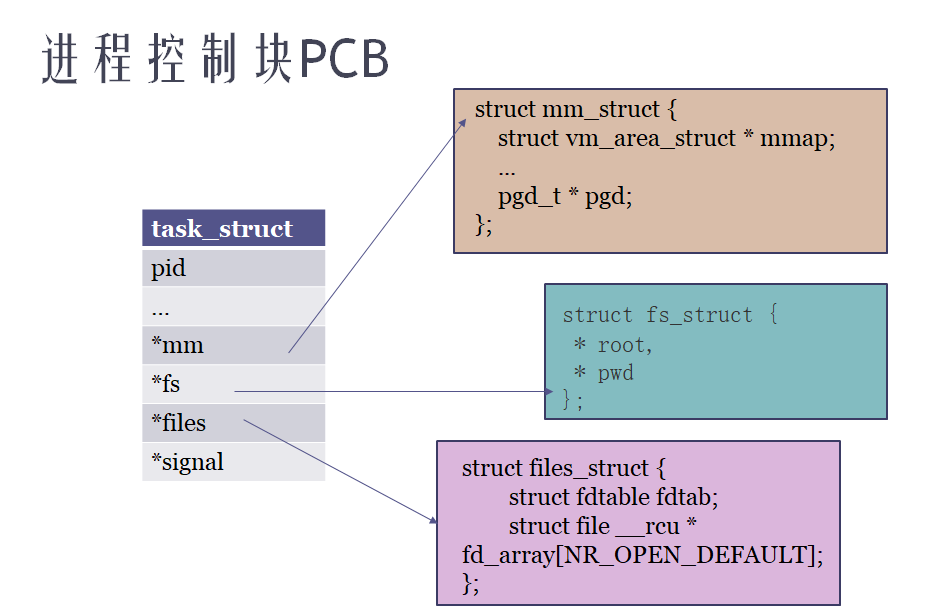
\includegraphics[width=9cm]{./figure/linux_pcb.png}
  \floatfoot{注:即linux中的task\_struct }
  }
\end{figure}
\begin{description}
  \item[\heiti{mm 内存资源:}] 进程的内存
  \item[\heiti{fs 文件系统资源1:}] 根路径和当前路径指针
  \item[\heiti{files 文件系统资源2:}] 进程打开的文件,文件描述符数组
  \item[\heiti{signal 信号资源:}] 不同进程可以针对同一信号挂不同的处理方法
  \item[\heiti{pid 属性资源:}] 描述进程的属性
\end{description}



\section{task\_struct的属性特点}
本节讲的主要是Pid属性是有限的这个特点,利用这个特点,实现linux下破坏死机和代码中破解的例子。
\subsection{fork炸弹让linux死机}
linux下著名的fork炸弹,一敲就让Linux死机。是利用不断利用fork产生进程把pid耗尽,其命令如下:
\begin{example*}
  \wdexpbox
  {\caption{fork炸弹}}
  {linux下著名的fork炸弹,一敲就让Linux死机。\\
  \textcolor[rgb]{1.00,0.00,0.00}{\#linux fork 炸弹}\\  
  \textcolor[rgb]{1.00,0.00,0.00}{\textbf{:()\{:\|:\&\};: } }
  }
\end{example*}

\begin{latexcmd}[label=linux fork 炸弹解析]
: 函数名为冒号

() 函数参数定义

{} 函数定义

:调用自己

|:递归调用自己

& 后台执行

; 函数结束

: 调用函数:
\end{latexcmd}

\subsection{pid数量限制导致安卓的一键root}
安卓的2.2.1之前的版本被发现一个漏洞,很容易就被一键root,安卓的调试软件adb刚开始时有root权限,之后adb调用api setuid(shell) 把自己从root用户降为shell用户。谷歌的工程师在调用时没有检查setuid的返回值,即默认setuid总是可以成功。黑客们利用uid数量有限制的属性,将shell用户内的pid进程全部用完,这样调用setuid时是无法成功的,但因为没有检查返回值,导致adb调用setuid(shell) 后没有降权成功,还是有root权限。这就是Android著名的提权漏洞:rageagainstthecage。2.2之后的安卓版本修复了此漏洞,方法是检查setuid的返回值。

查看Linux中最大Pid数量的命令如下:
\begin{lstlisting}[language={bash}]
wangfan@wangfan-VirtualBox:~$ ulimit -a
core file size          (blocks, -c) 0
data seg size           (kbytes, -d) unlimited
scheduling priority             (-e) 0
file size               (blocks, -f) unlimited
pending signals                 (-i) 15723
max locked memory       (kbytes, -l) 64
max memory size         (kbytes, -m) unlimited
open files                      (-n) 1024
pipe size            (512 bytes, -p) 8
POSIX message queues     (bytes, -q) 819200
real-time priority              (-r) 0
stack size              (kbytes, -s) 8192
cpu time               (seconds, -t) unlimited
max user processes              (-u) 15723
virtual memory          (kbytes, -v) unlimited
file locks                      (-x) unlimited
\end{lstlisting}

\subsection{linux的pid与tgid}
一个进程fork出子进程后,从linux内核的角度看,对应的pid肯定不一样。但是为了符合POSIX的标准要求,POSIX要求规定同一个父进程fork出的子进程,调用getpid返回的pid的号必须是一样的,我们用top命令查看进程可以看到fork出的子进程与父进程的Pid号是一样的。linux实现的原理就是通过增加一个tgid来实现父子进程调用getpid时返回值都一样的效果。
\begin{tcolorbox}[colback=blue!5,colframe=blue!75!black,title=pid和tgid 视频]
\videoattach{4- pid-tgid-pthread-self}{pid和tgid视频演示}
\end{tcolorbox}

\subsection{linux进程task\_struct的三种数据结构}
在linux代码中会涉及各种对task\_struct的引用关系,比如调度算法中会将task\_struct挂在链表上,父子进程的关系用树来描述,CFS调度算法会用到红黑树,通过pid查找进程则是用hash表的结构。其对应的数据结构如\ref{task_datastructure}所示

\begin{figure}[H]
 \wdfigbox
  {\caption{task\_struct汲及到的数据结构}\label{task_datastructure}}
  {
  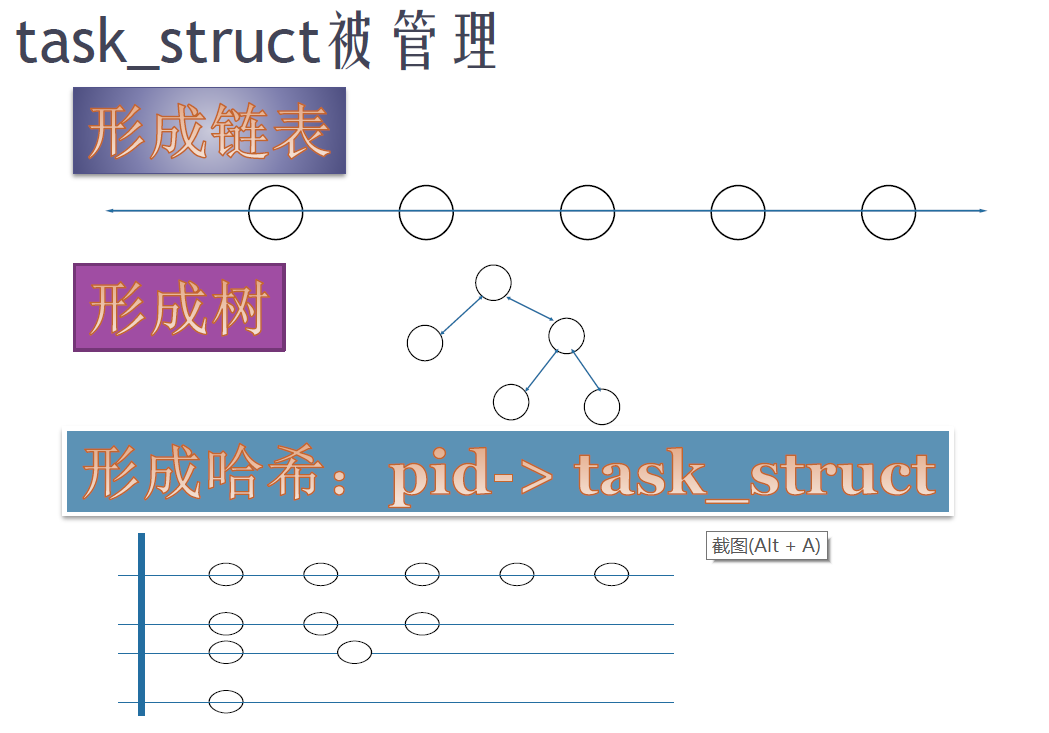
\includegraphics[width=9cm]{./figure/task_datastructure.png}
  \floatfoot{注: 每种数据结构选择都是根据应用场景的需求来选择实现目的效率最高的数据结构}
  }
\end{figure}
\chapter{进程的状态特征}
linux进程的生命周期对应6个状态,
\section{进程状态切换}
\subsection{进程运行时的3个基本状态}
操作系统包括实时系统对应进程一般都有3个状态,进程在有CPU时对应运行态,无CPU时对应就绪态和睡眠态。就绪态指所有资源都准备好,只要有CPU就可以运行了。睡眠指有资源还未准备好,比如读串口数据时,数据还未发送。此时有CPU也无法运行,需要等资源准备好后变成就绪态,然后得到CPU后才能变成运行态,其转换关系如\ref{process_3types}所示。

\begin{figure}[H]
 \wdfigbox
  {\caption{进程基本的三种状态转换}\label{process_3types}}
  {
  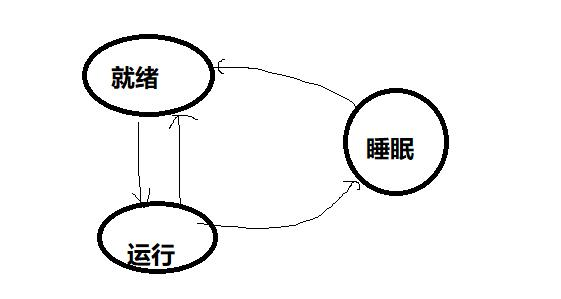
\includegraphics[width=9cm]{./figure/process_3types.jpg}
  \floatfoot{注:linux 除这三种状态外另外增加了状态}
  }
\end{figure}

\subsection{linux进程扩展的6个状态}

\begin{enumerate}
  \item {\heiti{僵尸态:}} 子进程退出后,所有资源都消失了,只剩下task\_struct,父进程在wait函数中可以得到子进程的死亡原因。在wait之前子进程的状态就是僵尸态。
  \item {\heiti{深度睡眠:}} 等待资源到位后才醒过来
  \item {\heiti{浅度睡眠:}} 等待资源到位或收到信号后都会醒过来
  \item  {\heiti{暂停:}} stop状态是被外部命令作业控制等强制进程进入的状态。
  \item  {\heiti{就绪:}} 未占用CPU,等待调度算法调度到运行态的进程
  \item  {\heiti{运行:}} 占有CPU,正在运行的线程。
\end{enumerate}

\begin{figure}[H]
 \wdfigbox
  {\caption{linux 进程6种状态转换}\label{linux_process_6types}}
  {
  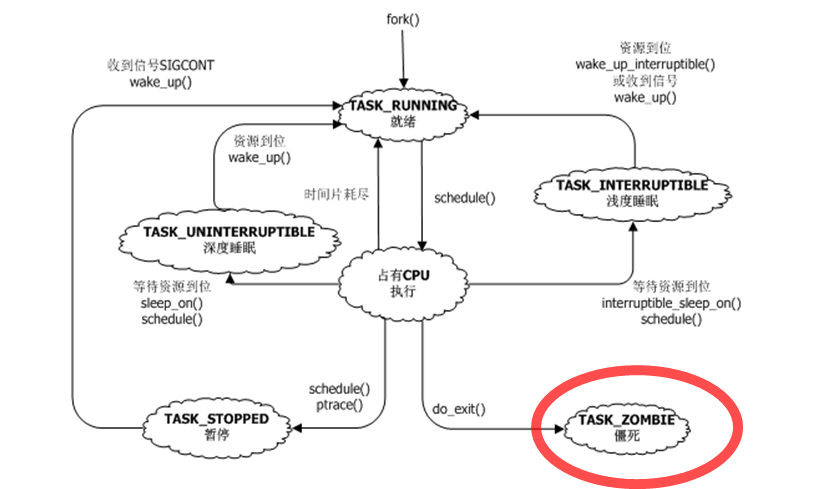
\includegraphics[width=9cm]{./figure/linux_process_6types.png}
  \floatfoot{注:linux 进程的运行转换图}
  }
\end{figure}
暂停状态是进程在运行过程中,通过外部bash命令强制让进程进入的状态。通过这种方法可以指定进程的CPU占用率。后面我们通常用cgroup的方法来实现,这里仅作了解。
\begin{latexcmd}[label=进入stop状态的方法]
作业控制的命令
ctrl + z, fg/bg
cpulimit
cpulimit -l 20 -p 10111
限制pid 为10111程序的CPU使用率不超过20%  
\end{latexcmd}
\subsection{linux进程状态的联系和区别}
\begin{description}
  \item[{\heiti{就绪VS运行}}] linux的调度算法只管理就绪和运行态中的进程,只对应\label{linux_process_6types}中的就绪和占有状态的进程,这两个状态都称为task\_running。
  \item[{\heiti{深度睡眠VS浅度睡眠}}] 深度睡眠只有资源到位才醒,收到信号也不醒,浅度睡眠资源到位或收到信号都会醒
  \item[{\heiti{睡眠VS暂停}}] 睡眠是代码中未得到资源主动进入的状态,暂停是程序外部强制进程进入的状态。
\end{description}


\section{进程的内存泄露}
内存泄露指随着时间的增长,进程的内存使用呈现线性增长的情况,指的是进程一直在运行,运行中申请了内存,但使用完后并没有释放,运行期间每次都申请内存而不释放导致系统内存越来越少的情况。这里要理解内存泄露的原因不可能是进程死了,内存没释放。因为进程死了之后就变成僵尸,Linux会自动将进程中申请的资源全部释放,只留下task\_struct让父进程wait来查看状态。不可能再占用内存。
%%% Local Variables:
%%% TeX-master: "main"
%%% End:



\partabstractfp{进程资源是如何处理的?进程与进程间是怎样的关系?进程死亡后会不会内存泄露?不同生命周期下进程资源的处理方式有什么差异?}
\partabstractrp{注:本章的架构是我根据讲课记录自己的理解划分的,可能与讲课不一致,如有错误欢迎指正。子死父收尸章节应该是第一天讲的,为了保持架构的一致性,把它挪到此处进行处理。}
\partabstractlettrine{从}{出生到死亡,生,死,睡过程} % the first word of the abstract

\part{进程课第2天}

\chapter{进程出生}
\section{进程出生时资源处理}
fork出子进程后,子进程的资源就直接从父进程的进程结构task\_struct拷贝出同样的信息,如\ref{child_fork_task_struct}所示。进程P2刚创建后,其资源是一模一样的。

\begin{figure}[H]
 \wdfigbox
  {\caption{fork子进程资源拷贝}\label{child_fork_task_struct}}
  {
  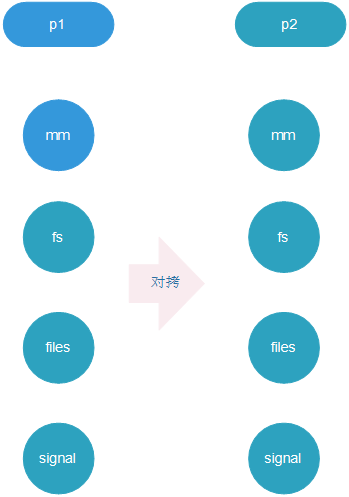
\includegraphics[width=8cm]{./figure/child_fork_task_struct.png}
  \floatfoot{注:所有资源结构体都进行拷贝  }
  }
\end{figure}
之后随着进程变化,本着谁修改谁分裂的原则进行资源变化的处理。

\section{进程分裂时的资源变化 -- COW}
父子进程刚诞生时所得到的资源是一样的,那这些资源在何时发生变化,以及变化后有什么影响,这就涉及到了linux的copy-on-write技术,下面通过 具体的实例来说明父子进程的资源变化流程。\\
COW(copy-on-write)技术是进程fork时采用的,涉及到虚拟内存和实际内存的映射关系。采用了COW技术后,进程处理会有一些现象需要重点注意。比如fork之后的父子进程读写同一个全局变量时,一个变量在不同的进程会显示出不同的值。
\subsection{COW 现象代码}
\begin{lstlisting}[language={C}]
#include <stdio.h>
#include <sys/types.h>
#include <unistd.h>
int data = 10;
int child_process()
{
    printf("child process %d, data %d\n", getpid(), data);
    data = 20;
    printf("child process %d, data %d\n", getpid(), data);
    _exit(0);
}
int main(int argc, char * argv[])
{
    int pid;
    pid = fork();
    if(pid == 0){
        child_process();
    }
    else{
        sleep(1);
        printf("parent process %d, data %d", getpid(),data);
        _exit(0);
    }
    return 0;
}
\end{lstlisting}
在正常情况下,程序修改全局变量data,再打印data,会是修改后的值 20,代码中子进程修改全局变量为20后,父进程等待1s,确保子进程已修改完成,但父进程最终打印的结果还是10。
\begin{latexcmd}[label= COW现象]
#运行程序的显示结果如下
child process 9491, data 10
child process 9491, data 20
parent process 9490, data 10
\end{latexcmd}

下面我们具体分析程序背后采用COW的原理和流程。\\
\subsection{COW 实现技术原理}
fork进程前后的内存关系如\ref{linux_fork_mem_compare}所示,
\begin{description}
  \item[\heiti{fork前第1阶段:}] 全局变量data对应数据段内存vir和phy都在数据段,权限为可读可写。
  \item[\heiti{fork后:}] vir和Phy的权限全部变成只读权限,读内存正常,写内存会进入page fault缺页中断。
  \item[\heiti{fork后写内存:}] 写内存后,发生缺页中断,Linux会重新申请一个4k内存,将新物理内存指向更改了内存地址的进程vir。同时将老的4k内存拷贝给新的内存,同时将权限改为R+W,这样父子进程的同一个vir虚拟地址就分别对应2个独立的可读可写的物理地址。总之谁先写谁拿到新的物理内存,原内存留给剩下的进程。
\end{description}
\begin{figure}[H]
 \wdfigbox
  {\caption{fork进程前后内存映射关系}\label{linux_fork_mem_compare}}
  {
  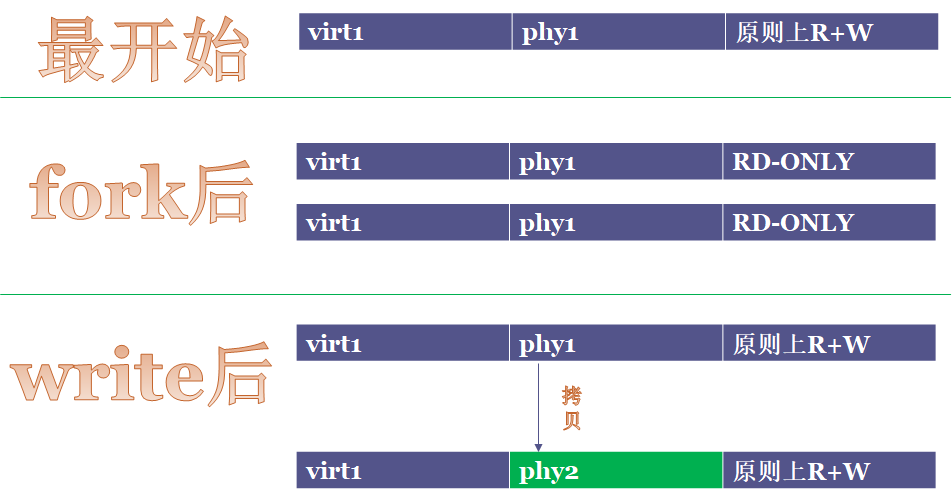
\includegraphics[width=9cm]{./figure/cow_fork_virmem_compare.png}
  \floatfoot{注:第一列为虚拟地址,第二列为物理地址,最后一列对应内存的读写权限 }
  }
\end{figure}
\subsection{无法用COW的情况:VFORK}
COW技术必须借助MMU(内存管理单元)来实现。COW是通过改变虚拟内存和物理内存的映射关系来实现,没有MMU的系统,无法实现虚拟内存和物理内存的映射。也无法调用fork函数,无MMU系统对应调用的是vfork函数,其资源变化对比fork如\ref{vfork_mem}所示:
\begin{figure}[H]
 \wdfigbox
  {\caption{vfork进程内存}\label{vfork_mem}}
  {
  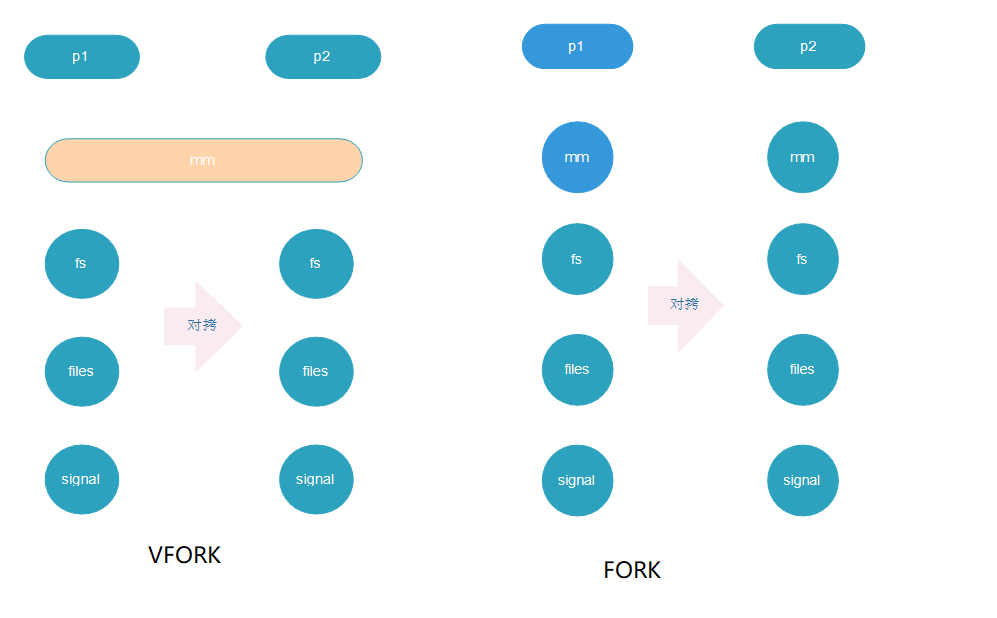
\includegraphics[width=10cm]{./figure/vfork_mem.png}
  \floatfoot{注:mm为同一份,没有进行拷贝  }
  }
\end{figure}
vfork的特点:vfork会阻塞父进程,只有等子进程完全退出后才执行父进程。vfork特性演示视频如下所示:

\begin{tcolorbox}[colback=blue!5,colframe=blue!75!black,title=vfork 视频]
\videoattach{2- vfork.avi}{vfork与COW区别}
\end{tcolorbox}

\subsection{强制共享资源--线程}
当P1和P2都用同一个资源,资源结构体不进行拷贝,P2的资源指针直接指向P1,这样就体现出线程的特征:可以调度又共享一样的资源。Linux中也是这样来实现线程的,调用pthread\_create时,会调到CLONE的API,这样就会让P2的资源指针指向P1。
\begin{figure}[H]
 \wdfigbox
  {\caption{线程资源处理}\label{thread_mem}}
  {
  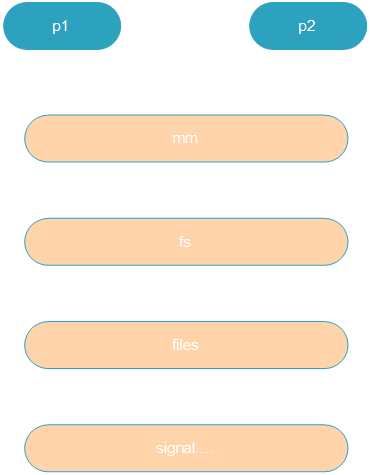
\includegraphics[width=4cm]{./figure/thread_resource.png}
  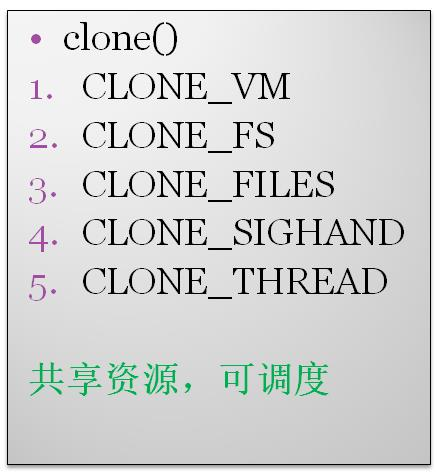
\includegraphics[width=4cm]{./figure/clone_api.jpg}
  \floatfoot{注:最终调用的API为CLONE,pthread\_create  }
  }
\end{figure}
\begin{tcolorbox}[colback=blue!5,colframe=blue!75!black,title=thread 视频]
\videoattach{3- thread.avi}{thread视频演示}
\end{tcolorbox}

\section{第1个进程,进程0与进程1}
开机后进程0创建出进程1,开机后进程0会退化成idle进程,idle进程的优先级最低。此进程运行的原则是所有其他的进程不运行时它就开始运行,当运行idle进程时,cpu就设置成低功耗模式。(注:与开机键中的suspend的区别是idle状态时只有cpu是低耗,suspend时显示器电源等其他设备也会进入低功耗)。此设计的精妙之处在于,如果不用进程0,进程进入低功耗模式的判断标准就变成了所有进程退出后要检查一下是否是最后一个进程,如果是最后一个就进入低功耗模式。这样的设计就会把检查状态耦合到了每个进程之中。增加进程0设计的好处在于,设计就简化只要判断是否在idle进程就可以了。实现了去耦合。
视频演示如下:
\begin{tcolorbox}[colback=blue!5,colframe=blue!75!black,title=idle进程视频]
\videoattach{7- idle-process.avi}{idle进程视频演示}
\end{tcolorbox}

\chapter{进程运行}
~\\程序运行时大部分进程状态为运行或睡眠。调度算法解决可以跑的运行状态(就绪和运行),剩下的不可以跑的进程就是睡眠和等待。睡眠实现对应的代码就是调用了schdule函数,唤醒则是对应的是schdule返回。一个进程等资源就会去睡,linux所有的睡眠,对应的task\_struct就会挂在队列wait\_queue上,当资源来了后,就会唤醒等待队列上的进程。视频演示如下:
\begin{tcolorbox}[colback=blue!5,colframe=blue!75!black,title=等待队列视频]
\videoattach{6- sleep-waitqueue.avi}{进程等待队列视频演示}
\end{tcolorbox}


\chapter{进程死亡}
fork执行后,就会变成2个进程返回,而不是一个进程返回两次。两个进程用的是同一段代码,不同的是在判断fork的返回值后会走向不同的分支。子进程返回的是0,则if(pid == 0)后执行的是子进程,父进程接收到的返回值是子进程的pid值。如下所示:

\dirtree{%
.1 fork之后.
.2 返回值为-1\DTcomment{fork失败}.
.2 返回值为0\DTcomment{子进程返回}.
.2 返回值为pid号\DTcomment{父进程返回}.
}

\section{子死父收尸}
linux中子进程死亡时首先变成僵尸,父进程通过wait来获取子进程的死亡原因。调用的API如\ref{child_wait}所示,父进程通过分析子进程的退出码就可以知道具体的退出原因了。

\begin{figure}[H]
 \wdfigbox
  {\caption{子进程死亡原因获取}\label{child_wait}}
  {
  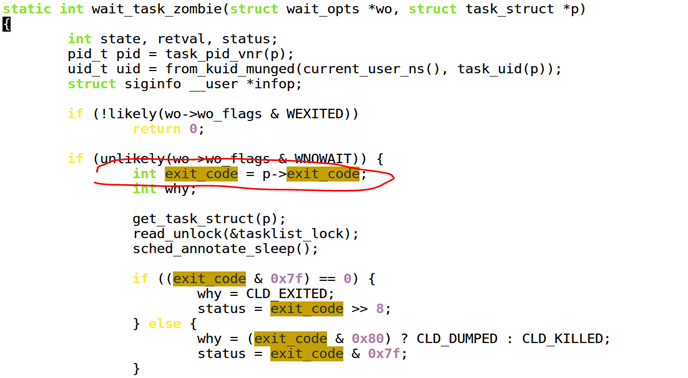
\includegraphics[width=10cm]{./figure/child_wait.png}
  \floatfoot{父进程通过exit\_code获取子进程退出信息}
  }
\end{figure}

\begin{tcolorbox}[colback=blue!5,colframe=blue!75!black,title=子进程死亡原因获取视频]
\videoattach{1- child-waited-by-parent.avi}{父进程获取子进程死亡原因视频演示}
\end{tcolorbox}
\section{父死子托孤}
任何一个进程死亡后有个原则,首先托付给subreaper,如果没有subreaper则托付给init。如\ref{child_process_died}所示。进程可以通过API来设置自己为subreaper。subreaper要注意调用wait来处理可能托付过来的僵尸进程。
\begin{figure}[H]
 \wdfigbox
  {\caption{进程死亡后挂接关系}\label{child_process_died}}
  {
  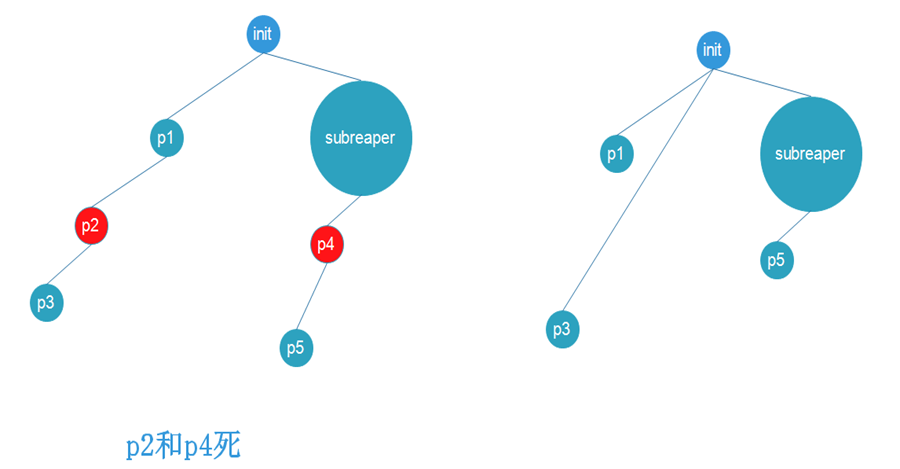
\includegraphics[width=10cm]{./figure/child_process_died.png}
  \floatfoot{挂到init或subreaper  }
  }  
\end{figure}

\begin{tcolorbox}[colback=blue!5,colframe=blue!75!black,title=进程托孤视频]
\videoattach{5- orphan.avi}{进程托孤视频演示}
\end{tcolorbox}
\clearpage
%%% Local Variables:
%%% TeX-master: "main"
%%% End:




\partabstractfp{\textbf{进程第3天课程摘要}}
\partabstractrp{本章讲述如何根据不同类型的进程分配不同策略的调度算法,调度算法的原理及应用对象。还有如何更改进程的调度策略}
\partabstractlettrine{类}{型不同,策略不同。} % the first word of the abstract

\part{进程课第3天}
\chapter{进程分类}
\section{CPU消耗}
 
\section{IO消耗型}

\section{arm大小核设计}
\begin{example*}
  \wdexpbox
  {\caption{ARM的big.LITTLE设计}}
  {采用大核+小核的设计,大核功耗高,运算力强,用于处理CPU消耗性任务,小核功耗低,功耗小,用于处理I/O消耗性任务。实现功耗降低,但处理效果与全是大核处理一致的效果}
\end{example*}

\chapter{进程调度策略}
\section{RT进程调度}
\subsection{SCHED\_FIFO}
\subsection{SCHED\_RR}


\section{NORMAL进程调度}
\subsection{CFS调度}
\clearpage


\chapter{调整优先级}
\section{用 renice 改变进程优先级}
\section{用 nice 改变进程优先级}
\section{用 chrt 改变进程优先级}
\clearpage
%%% Local Variables:
%%% TeX-master: "main"
%%% End:



\partabstractfp{\textbf{进程第4天课程摘要} 这里讲的是CPU处理的负载,对应负载指CPU处理的任务\\
1. linux的4种不同优先级任务是什么\\
2. 不同优先级任务间的抢占原则是什么?\\
3. 负载均衡的不同类型及使用方法。}
\partabstractrp{1. 实时系统是什么?\\
2.linux 为什么不是一个硬实时系统?\\
3.linux RT实时补丁的原理,使用方法及限制。}
\partabstractlettrine{负}{载均衡} % the first word of the abstract

\part{进程课第4天}


\chapter{负载均衡}
\textattachfile{0 - IO-CPU.avi}{\textcolor[rgb]{0.00,0.00,0.55}{\textbf{CPU测试}}}
\chapter{实时系统}
%%% Local Variables:
%%% TeX-master: "book_template_2"
%%% End:




\partabstractfp{\textbf{进程问题集锦} }
\partabstractrp{}
\partabstractlettrine{F}{AQ,本章记录课间和课后宋老师与我们之间的问题} % the first word of the abstract

\part{进程问题集锦}


\chapter{}
%%% Local Variables:
%%% TeX-master: "main"
%%% End:



\partabstractfp{}
\partabstractrp{参考的文件以PDF附件的形式,可以双击链接打开或保存,需选择支持PDF附件的PDF阅读器,建议使用adobe的阅读器打开附件}
\partabstractlettrine{参}{考这章列举了用到的相关资料源地址} % the first word of the abstract
\part{参考资料}
\chapter{参考文献}
\section{宋宝华相关网站资源}
\begin{enumerate}
  \item \href{https://edu.csdn.net/course/detail/5995}{CSDN视频课程 打通Linux脉络系列:进程、线程和调度}
  \item linux公众号:\textbf{Linux阅码场}
\end{enumerate}

\section{相关文章网址}
\begin{enumerate}
  \item \href{https://blog.csdn.net/feglass/article/details/46403501}{Android提权漏洞分析——rageagainstthecage}
  \item \href{https://github.com/21cnbao/training/blob/master/kernel/drivers/globalfifo/ch12/globalfifo.c}{globalfifo.c github源码地址}
  \item 
\end{enumerate}

\chapter{相关附件}
\section{pdf课件}
4天课程的PPT讲义,请用支持PDF附件的阅读器打开本文档,双击打开附件或在附件中另存为处理。
\begin{enumerate}
  \item \textattachfile{process_schedule_lesson1.pdf}{\textcolor[rgb]{0.00,0.00,0.55}{\textbf{第1天进程讲义PDF}}}
  \item \textattachfile{process_schedule_lesson2.pdf}{\textcolor[rgb]{0.00,0.00,0.55}{\textbf{第2天进程讲义PDF}}}
  \item \textattachfile{process_schedule_lesson3.pdf}{\textcolor[rgb]{0.00,0.00,0.55}{\textbf{第3天进程讲义PDF}}}
  \item \textattachfile{process_schedule_lesson4.pdf}{\textcolor[rgb]{0.00,0.00,0.55}{\textbf{第4天进程讲义PDF}}}
\end{enumerate}



\section{视频文件}
\ifattachpdffile
\textattachfile{0 - IO-CPU.avi}{\textcolor[rgb]{0.00,0.00,0.55}{\textbf{0-IO-CPU}}}


\else
\videowarn
\fi
%%% Local Variables:
%%% TeX-master: "main"
%%% End:


%====== be sure to add this part ====%
%\addtocontents{toc}{\protect\end{multicols}}
\wdenddoc
%====== be sure to add this part ====%

%\enddoc

\end{document}
